% -*- coding: utf-8 -*-
% !TEX encoding = UTF-8 Unicode
% !TEX root =  main.tex

\chapter{Theoretische und begriffliche Grundlagen}\label{cha:grundlagen}

Um auf die Regelung einer anisotropen Synchronmaschine einzugehen, werden im folgenden einige Grundlagen erörtert.

\section{Theorie der Drehfeldmaschinen}\label{sec:grund-drehfeld}

Drehfeldmaschinen sind die am häufigsten eingesetzten Antriebsmaschinen, der Grund hierfür ist die Robustheit der aktiven Bauteile und die gute Energieeffizienz.
Zudem besitzen Drehfeldmaschinen ein großes Leistungsspektrum und einen großen Drehzahl- und Drehmomentstellbereich.
Die wesentlichen Vertreter der Maschinenfamilie sind die Synchron- und die Asynchronmaschinen.
Beide basieren auf der Wirkung eines Drehfeldes, das sich durch den Luftspalt der Maschine bewegt.

\subsection{Magnetfelder}

\subsubsection{•}



\section{Allgemeine Grundlagen der Drehstrommaschinen}\label{sec:drehstrommaschinen}

Die Synchron- und Asynchronmaschine besitzen im Ständer denselben Aufbau und erfordern zur Darstellung ihres Verhaltens eine Reihe gleicher physikalischer Begriffe.
Es ist zweckmäßig die Grundlagen der Synchronmaschine in einem eigenen Kapitel zu behandeln.
Dies gilt \insb für den Aufbau der Drehstromwicklungen sowie die Grundlagen zu Beschreibung von umlaufenden Durchflutungen und deren Felder.

\subsection{Drehstromwicklungen}

Der prinzipielle Aufbau einer Drehstromwicklung lässt sich anhand aus den Anforderungen zur Erzeugung einer dreiphasigen Wechselspannung erläutern.
Eine solche Drehspannung erhält man mit einer Anordnung nach \autoref{fig:drehstromwicklung}.
Ein aus Dynamoblechen geschichtetes Ständerblechpacket enthält in Nuten am Bohrungsumfang gleichmäßig verteilte Leiter, die zu drei räumlich verteilten Wicklungssträngen zusammengeschaltet werden \autocite[S.~141]{fischer2009}.
Der Läufer erzeugt ein Gleichfeld, das eine sinusförmige Feldverteilung längst des Luftspaltes aufbaut.
Hat der Läufer eine konstante Drehzahl, so induziert das Feld in den einzelnen Spulen zeitlich sinusförmige Spannungen, die sich innerhalb eines Wicklungsstranges zu einem Wert addieren.
Die Berechnung der Induktion kann über die Allgemeine Beziehung

\begin{align}
u_q = B\cdot l \cdot v
\end{align}

erfolgen.
Sei $d_1$ der Bohrungdurchmesser des Ständerblechpaketes einer $2p$-poligen Maschine, so bezeichnet man den Umfangsanteil

\begin{align}
\tau_p = \frac{d_1 \cdot \pi}{2p}
\end{align}

wieder als Polteilung.
Die Polteilung entspricht der Länder einer Halbwelle der sinusförmigen Flussdichteverteilung im Luftspalt (enspricht einem elektrischen Winkel von $\omega t = 180^{\circ}$.
Bei einer zweipoligen Maschine mit $p=1$ stimmen somit der räumlich mechanische und der elektrische Winkel überein, allgemein gilt die Beziehung \autocite[S.141f.]{fischer2009}

\begin{align}
\gamma_{el} = p\cdot \gamma_{mech}
\end{align}



\begin{figure}[!htb]
\centering
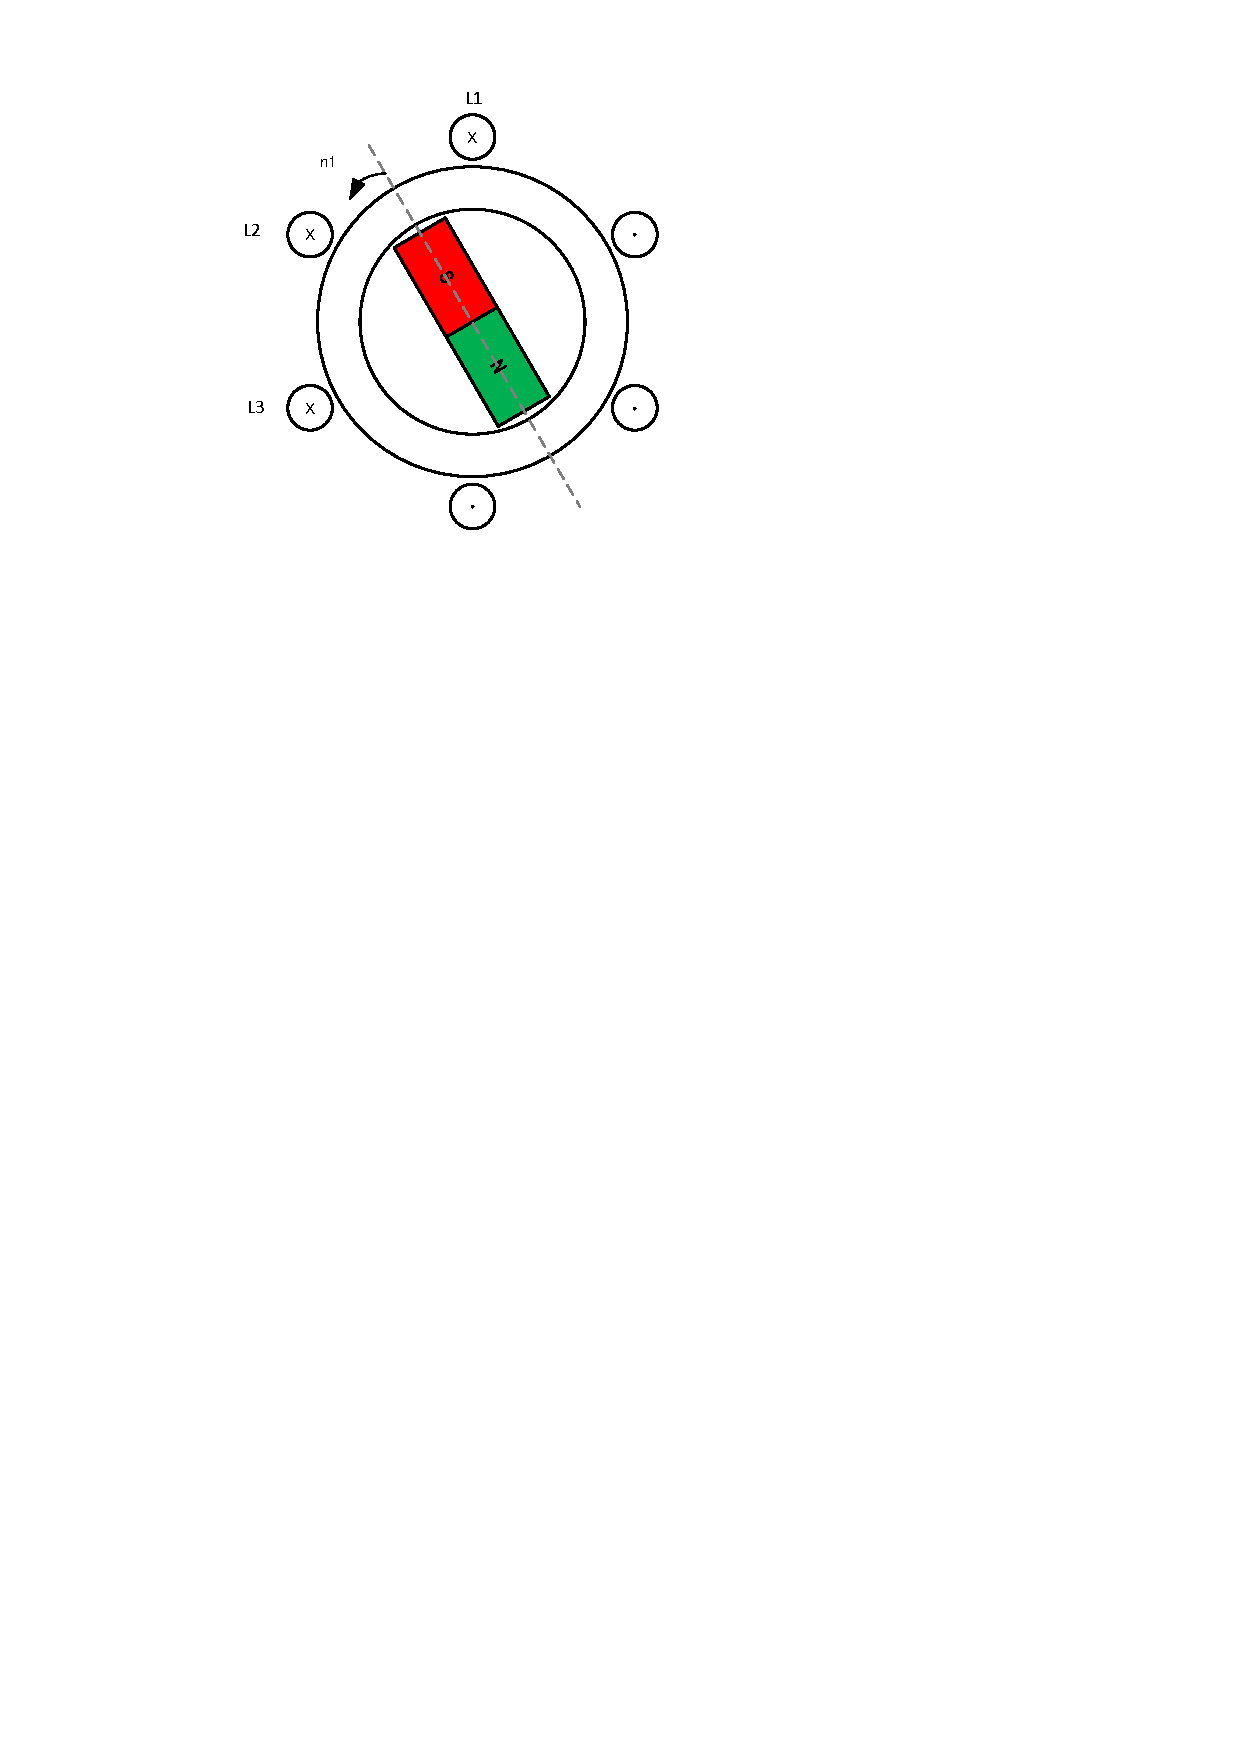
\includegraphics[width=0.5\textwidth]{Visio-synchronmaschine-drehstrom.pdf}
\label{fig:drehstromwicklung}
\caption{Erzeugung einer mehrphasigen Spannung durch ein räumlich sinusförmiges Läuferdrehfeld in Anlehnung an \autocite[S.~141]{fischer2009}}
\end{figure}

\section{Induktivitäten}\label{sec:induktiv}

\section{Einführung Synchronmaschine}\label{sec:synchron}

\paragraph{Historischer Hintergund} Die ersten Synchronmaschinen wurden als Einphasengenerator entwickelt und gebaut, den ersten dreiphasigen Synchrongenerator entwickelten 1887 unabhängig voneinander F.~A.~Haselwander\footnote{Friedrich August Haselwander war ein deutscher Ingenieur, ein Erfinder der Drehstrom-Synchronmaschine und des kompressorlosen Ölmotors.} und C.~S.~Bradley\footnote{Charles Schenk Bradley war ein US-amerikanischer Elektrotechniker, Erfinder und Pionier von frühen Elektromotoren. Er zählt neben F.~A.~Haselwander zu den Begründern des heute im Bereich der elektrischen Energietechnik eingesetzten Dreiphasenwechselstromes.} Bei den Entwicklungen bildeten sich die Bauformen der Schenkelpol- und Vollpolmaschine aus. Die Weiterentwicklung der Synchronmaschine hing stark mit dem Ausbau der Energieversorgung und dem Bedarf von leistungsstärkeren Generatoren zusammen. Unabhängig von der Entwicklung wurden schon sehr früh Synchronmaschinen als Antriebsmaschinen für eine konstante Drehzahlregelung oder einen Phasenbetrieb in der Industrie eingesetzt \autocites[S.~108f.]{ternes2012}[S.~287]{fischer2009}[S.~485f.]{mullerI2005}.

Die gleichstromgespeiste Erregerwicklung ermöglicht es, das Magnetfeld unabhängig vom Netz zu beeinflussen.
Als Spannungsquelle für die Speisung der Erregerwicklung wurden sog.\ Gleichstromerregermaschinen eingesetzt, in der heutigen Zeit werden Wechselspannung mit Hilfe von Leistungselektronischen Schaltungen gespeist.
Um die Schleifringübertragung der Erregerleistung zu umgehen, werden schleifring- bzw.\ bürstenlose Erregersysteme realisiert \autocite[S.~108]{ternes2012}.
Als Motor wurden Drephasen-Synchronmaschinen schon bald für große Leistungen eingesetzt, \zB zum Antrieb von Pumpen und Verdichten \autocite[S.~486]{mullerI2005}.
Der Nachteil ist, dass die Drehzahl durch die Netzfrequenz festgelegt ist.
Die Synchronmaschine arbeitet unabhängig von der Belastung stets mit der durch die Netzfrequenz und die ausgeführte Polpaarzahl festgelegten synchronen Drehzahl.

Heute ist es möglich mit Hilfe eines Frequenzumrichters die Drehzahl der Synchronmaschine zu steuern.
Aus diesem Grund werden größere Gleichstrommaschinen durch drehzahlvariable Synchronmaschinen abgelöst.
Im Bereich kleinerer Leistungen wird anstelle der Gleichstromerregung eine Erregung durch Permanentmagnete eingesetzt.
Dabei verliert man die Beeinflussung des Erregerzustandes über den Erregerstrom, dafür erhält man eine elektrische Maschine die keine elektrische Verbindung zum Läufer erfordert.


\subsection{Beschreibung der Synchronmaschine im dq-Koordinatensystem}

\begin{figure}[!htb]
\centering
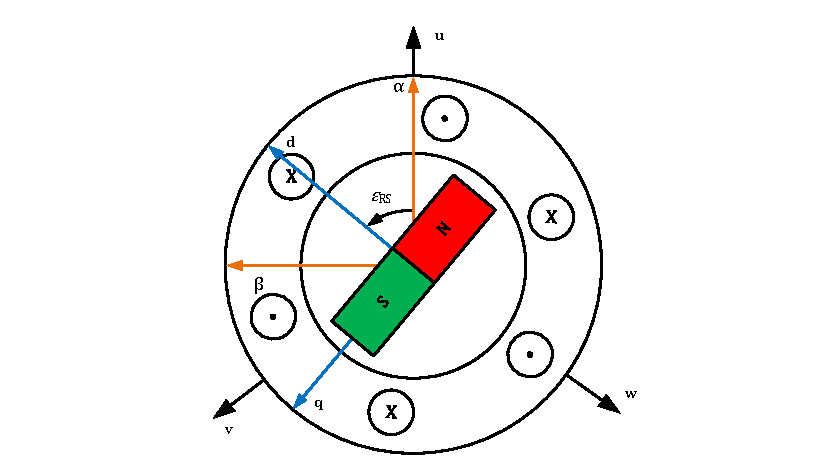
\includegraphics[width=\textwidth]{synchron-dq.pdf}
\label{fig:synchron-dq}
\caption{Darstellung der Synchronmaschine im dq-Koordinatensystem in Anlehnung an \parencite[S.~257]{schroeder2000}.}
\end{figure}

\section{Besonderheiten der Schenkelpolmaschine}\label{sec:schenkelpol}

\section{Permanenterregte Synchronmaschine}\label{sec:pmsm}

\section{Evalurierung der Ersatzschaltbilder für die Regelung}\label{sec:esb}

\begin{figure}[!htb]
\centering
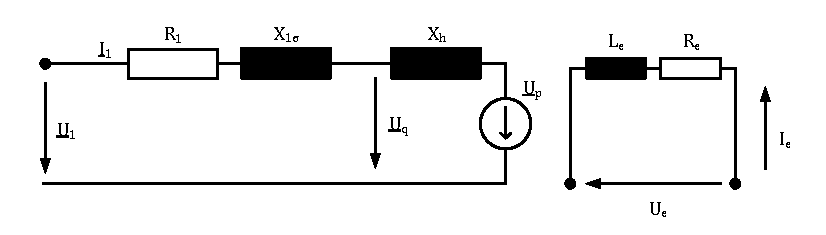
\includegraphics[width=\textwidth]{synchron-esb-kremser2004.pdf}
\label{fig:esb-kremser}
\caption{Ersatzschaltbild der Synchronmaschine nach \parencite[S.~145]{kremser2004}.}
\end{figure}

%%% Local Variables: 
%%% mode: latex
%%% TeX-master: "main"
%%% TeX-open-quote: "\\enquote{"
%%% TeX-close-quote: "}"
%%% LaTeX-csquotes-open-quote: "\\enquote{"
%%% LaTeX-csquotes-close-quote: "}"
%%% End: 

